\chapter{Original contribution to the solution of the problem}
This chapter presents the original contribution to the problem being studied. The research builds upon previous work in the field, but introduces a novel approach to addressing the challenges faced by current solutions. The specific problem being addressed and the ways in which the approach differs from existing methods are discussed. A detailed description of the proposed solution, including any new algorithms or techniques developed, is provided. Finally, an overview of the tools, technologies, and models used for the realization of the proposed solution will be presented in this chapter. The potential impact on the field and the expected outcomes of the proposed solution are also discussed.

\section{Definition of the proposed methodology}
The methodology proposed in this work consists in evaluating the application of anomaly detection techniques to the field of epileptic seizure prediction, by taking as starting points the two previous networks presented as reference works in sections \ref{subsec:refwork-uab} and \ref{subsec:refwork-unisa}.

In the first case the network, which is already an autoencoder applied for epileptic seizure detection, will be optimized and trained and tested for epileptic seizure prediction. The results will be then compared to those achieved by the work described in section \ref{subsec:refwork-siena} which was found to be one of the best performing experiment in the overall state-of-art.

In the second case the model used is a deep \gls{CNN} which was trained in a common supervised training setup, achieving results which are comparable to the state of the art, which are those obtained in the work of section \ref{subsec:refwork-siena}, as previously stated. An unsupervised anomaly detection adaptation of such work is presented, using the first layers of those pretrained models to translate the records in a smaller latent space that will than be submitted to a \gls{OC-SVM} classifier that should be able to generalize the meaning of normality/anormality in the subspace.

\subsection{Data grouping} \label{subsec:data-grouping}
In both cases the data used to train each instance of a model will be specifically selected to simulate real life scenarios of application of the network. These approaches according to which the experiment were conducted are patient specific, patient generic and inter-patient.

\subsubsection{Patient specific}
The patient specific approach represent the interaction that sees the patient receiving an \gls{EEG} headset associated to an untrained model. Over the course of a couple of days without incidents the system would than have gathered tens of hours of normal recording, thus having a comparable amount of recording data to that available in most public datasets accessible nowadays. Finally, the system could be train on this data to learn the specific representation of normality to the interested patient.

The downside of this approach is having to start the training phase from scratch, with the risk of not exploring many cases of borderline normality. For example the \gls{EEG} registered from a patient that is subject to strong emotional episodes or engaged in highly focused instances of study could present patterns substantially different to those obtained in everyday recordings.

\subsubsection{Patient generic}
The patient generic approach is associated to a scenario that would imagine the received \gls{EEG} headset being associated to a model previously trained on all the available \gls{EEG} instances available in a dataset. The system would then be completely ready to be used, without the need for further training sessions.

In this case the model would be trained on a fairly higher amount of recordings when compared to those available in the patient specific case, being the data gathered from multiple sources. Nonetheless, the model could be unable to learn a normality representation that is a good fit for the interested patient.

\subsubsection{Inter-patient}
The inter-patient approach is the only one that can be applied to both the networks in section \ref{subsec:refwork-uab} and \ref{subsec:refwork-unisa}, since in the second case the models used would pretrained with common supervised systems. 
This approach would take the patient generic one a step further by also including ideas from the patient specific scenario. In fact, the interested patient would receive an headset pretrained on data from many different sources, but the disadvantages would be mitigated by a second training phase, limiting the training data to those gathered from the current patient.

Ideally this method should be the best fit for a real world application, being it expected to perform better than the two previous methods when taken separately.

\subsection{Desired results}
% massimizzare specificity per minimizzare worrying time percentage max e average
In order to objectively determine the outcome of the experiments a clear assessment of the desired performance becomes mandatory.
It should be clear that close to state-of-art results would mean a successful application of the unsupervised anomaly techniques to the field of epileptic seizure prediction, but this would hardly translate to a possible usage of such technologies to real world scenarios unless those results are put in perspective.

For this reasons, the following goals have been identified with the aim of evaluating the overall improvements that these systems can make to the life of patients suffering from epilepsy:

\begin{itemize}
    \item Maximizing the interval between consecutive false positive detections, or \gls{IFP}
    \item Achieving an average prediction time that is short enough for the user to take due safety precautions, but sufficiently long so that the user would not wait too long after a falsely positive detection is issued before resuming his activities
\end{itemize}

From the combination of these equally important goals arises the need for the \gls{IFP} to be strictly greater than the maximum prediction time, or $t_p^M$. If it was not the case, a patient would be warned more frequently than the time he is expected to interrupt his activities as safety measures.
This idea is also expressible as a maximum worrying time percentage, or $t_w^M\%$, that is less than 100\%.

A desirable result would numerically be summarized by the following constraints:

\begin{equation} \label{eq:app-constraints}
    IFP > 24 h
    \quad\text{,}\quad 
    t_p^m > 30 s
    \quad\text{and}\quad
    t_w^M\% < 1\%
\end{equation}

The prediction accuracy is estimated to be of secondary importance because a system that does not satisfy the previous goals is unusable in principle. Nevertheless, achieving non-zero prediction accuracy is still, of course, mandatory.

\section{Methodological innovations}
In my thesis, I introduce several methodological innovations in the field of epileptic seizure prediction. 

One of the key contributions is the application of unsupervised deep anomaly detection techniques to this area of research. This approach is novel and has the potential to ease some of the problems that affect standard supervised techniques, such as the gathering of data. 

Additionally, I propose the use of different data grouping methods, such as patient-specific and patient-generic, to simulate real-life situations. The idea of inter-patient, which consists of refining models obtained from the patient-generic method, is an original idea that also has the potential to overcome the challenges of applying these findings in real-life situations. 

Another innovation is the use of models from slightly different scenarios that are known to work, as a way to evaluate more accurately the feasibility of applying this method. 

Finally, the evaluation of the results using real-life scenarios metrics, such as the worrying time percentage, is a new approach in this field. This allows for a more accurate assessment of the results and their impact on the lives of patients, as opposed to other studies that only claim their results are good enough without putting them into perspective.

\section{Design of the proposed system}
The design of the proposed system encompasses two distinct systems developed taking into account previous considerations. These systems will be described in detail in the following sections, highlighting their unique features and functionality.

\subsection{LSTM Autoencoder} \label{subsec:lstm}
The architecture and the number of parameters of the system are exactly the same as those presented in a previous section: \ref{subsec:refwork-uab}.

The system is trained with the goal of minimizing the reconstruction error, calculated as the \gls{MSE} between the input and output of the network. The \gls{MSE} loss function is used for this purpose. 
The trained system's output is thus a sequence that is similar to the input. To identify anomalies, the reconstruction error with \gls{MSE} is checked, and when it is above a threshold, the sample is considered anomalous and preictal, otherwise normal and interictal. 

To find the threshold, a validation set is used and the maximum reconstruction error is taken, with the aim of maximizing specificity. The idea is that the maximum value of the \gls{MSE} loss on the validation set is less than the maximum reconstruction error for preictal samples and greater than all interictal loss. Since outliers may be present in the validation set that would prevent recognizing truly positive samples, it is possible to avoid choosing the maximum error as the threshold and use a percentile close to 100\%, such as 99.9\% or 99.8\%.

\subsection{CNN and OC-SVM} \label{subsec:cnn}
In this case, the first part of the architecture consists of the feature extraction component of the network described in the previous section \ref{subsec:refwork-unisa}, up to the flatten layer, as depicted in the accompanying Fig. \ref{fig:cnn-feature-extractor}.

\begin{figure}[ht]
    \centering
    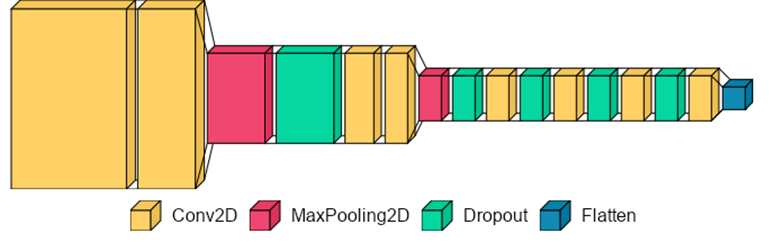
\includegraphics[width=1.0\textwidth]{images/Contribution/cnn-feature-extractor.png}
    \caption{The feature extraction half of the network as described in section \ref{subsec:refwork-unisa}}
    \label{fig:cnn-feature-extractor}
\end{figure}

The feature extractor transforms the windows into a lower dimensional subspace. This subspace is then subjected to an \gls{OC-SVM} with the goal of learning the concept of normality in this feature space, as shown in Fig. \ref{fig:cnn-anomaly-detector-architecture}. The idea is that since the feature extractor has been able to bring the data into a space where the \gls{MLP} classifier was able to learn to separate interictal from preictal in a supervised learning setup, unsupervised anomaly detection methods could also be capable of finding zones of normality in the same subspace.

\begin{figure}[ht]
    \centering
    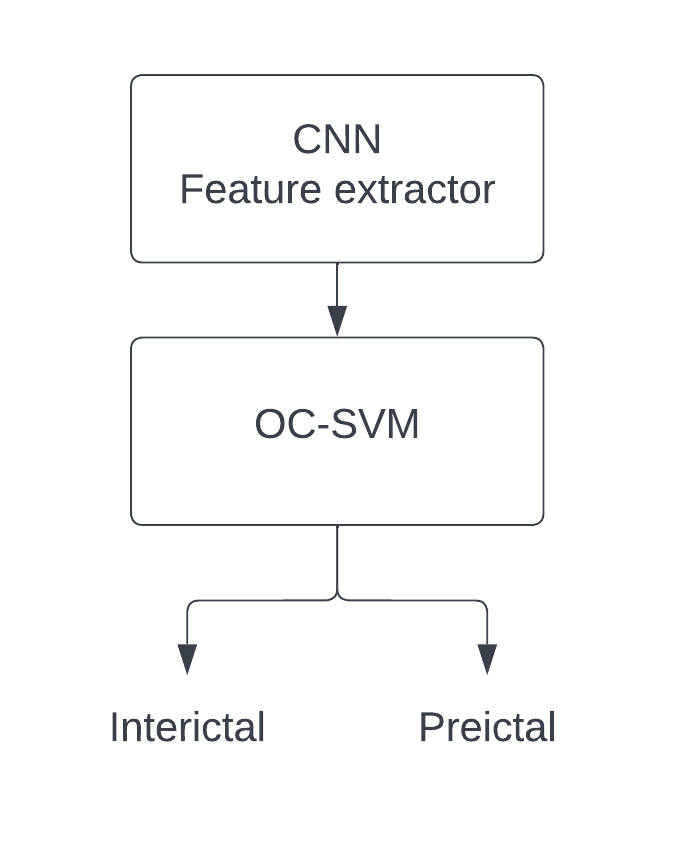
\includegraphics[width=0.5\textwidth]{images/Contribution/cnn-anomaly-detector-architecture.png}
    \caption{\gls{CNN} feature extractor into \gls{OC-SVM}}
    \label{fig:cnn-anomaly-detector-architecture}
\end{figure}

The feature extractor will be trained in a supervised manner with the rest of the original network, while the \gls{OC-SVM} will be trained separately in an unsupervised manner on data from patients unseen during the first training phase.

\section{Tools, technologies and models used for the realization}
The project was developed using Python and different libraries. MNE, an open-source Python library, was utilized for EEG signal visualization, processing and analysis. NumPy and SciPy were used for data processing and generating spectrograms. Pytorch and SciKit-learn were employed during the training and testing phase. Additionally, Seaborn and Matplotlib were used to create charts, Pandas was used to manage data, and h5py was used to store the data.

The training were GPU accelerated using the Nvidia Titan X Pascal kindly provided by the Department of Information and Electrical Engineering and Applied Mathematics and an Nvidia RTX 3090 personally owned by the candidate.